\documentclass{tudelft-report}

%% Set up the bibliography
\usepackage[style=apa]{biblatex}
\addbibresource{report.bib}

%% Additional packages and commands
\usepackage{parskip}
\setlist{itemsep=-2pt} % Reducing white space in lists slightly
\renewcommand{\deg}{\si{\degree}\xspace} % Use \deg easily, everywhere
\usepackage{booktabs}
\usepackage{siunitx}
\usepackage{graphicx}
\usepackage{acronym}
\usepackage{tabularx} 
\usepackage{float}
\usepackage{subcaption}
\usepackage{todonotes}
\usepackage{tablefootnote}

%% ----------------------------------------------------------------------
%%    Begin of document + Frontmatter (Roman page numbering)
%% ----------------------------------------------------------------------

\begin{document}

\frontmatter

%% Define the main parameters
\title{MIMOSA}
\subtitle{MIssion to Mars with a sOlar sAil}
\author{I. Gallo López}

\subject{AE4889: Special Topics in Astrodynamics} % Cover only
\affiliation{Delft University of Technology} % Cover only
\coverimage{figures/cover_gemini.png} % Aspect ratio of 2:3 (portrait) recommended
\definecolor{title}{HTML}{4884d6} % Color for cover title

\makecover

\begin{titlepage}

\begin{center}

%% Print the title
{\makeatletter
\largetitlestyle\fontsize{45}{45}\selectfont\@title
\makeatother}

%% Print the subtitle
{\makeatletter
\ifdefvoid{\@subtitle}{}{\bigskip\titlestyle\fontsize{20}{20}\selectfont\@subtitle}
\makeatother}

\bigskip
\bigskip

by

\bigskip
\bigskip

%% Print the name of the author
{\makeatletter
\largetitlestyle\fontsize{25}{25}\selectfont\@author
\makeatother}

\bigskip
\bigskip

%% Student details and personal problem specification
\setlength\extrarowheight{4pt}
\begin{tabular}{ll}
    \textbf{Student name}   & Ismael Gallo López \\
    \textbf{Student number} & 6541356 \\
    \textbf{Repository link} & \url{https://github.com/ismaelgallolopez/MIMOSA-special-topics-astrodynamics}\\\midrule
    \multicolumn{2}{l}{\textbf{Personal problem specification}} \\[2pt]
    Sun/Earth Lagrange point            & L2 \\
    Sun/Mars Lagrange point             & L2 \\
    Shift in Lagrange points {[-]}      & 0.00100 \\
    Radius Martian parking orbit {[km]} & 244{,}444 \\
    Lightness number {[-]}              & 0.0300 \\\midrule
    \textbf{Collaborated with} & Rodrigo Duarte Soares \\
     & Pablo García-Conde Ortiz \\
     & Nicolò Basso \\
\end{tabular}

\vfill

%% Print some more information at the bottom
\begin{tabular}{ll}
    Responsible Instructor:       & Dr.ir. M.J. Heiligers \\
    Teachers: & O. Celik; F. Gámez Losada; A. Minervino Amodio \\
    Project Duration: & April, 2026 -- June, 2026 \\
    Faculty:          & Faculty of Aerospace Engineering, Delft
\end{tabular}

\bigskip
\bigskip

%% Add a source and description for the cover and optional attribution for the template
\begin{tabular}{p{15mm}p{10cm}}
    Cover: & Image generated by the author using Google Nano Banana (Gemini 2.5 Flash Image). \\
\end{tabular}

\end{center}

%% Insert the TU Delft logo at the bottom of the page
\begin{tikzpicture}[remember picture, overlay]
    \node[above=10mm] at (current page.south) {%
        
\includegraphics{figures/logo-black}
    };
\end{tikzpicture}

\end{titlepage}
% \chapter*{Preface}
\addcontentsline{toc}{chapter}{Preface}

\emph{A preface...}

\begin{flushright}
{\makeatletter\itshape
    \@author \\
    Delft, \monthname{} \the\year{}
\makeatother}
\end{flushright}

% \chapter*{Summary}
\addcontentsline{toc}{chapter}{Summary}

\emph{A summary...}


\tableofcontents
%\listoffigures
%\listoftables

\chapter*{Acronyms}
\addcontentsline{toc}{chapter}{Acronyms}

\begin{acronym}[CR3BP]
  \acro{cr3bp}[CR3BP]{Circular Restricted Three-Body Problem}
  \acro{srp}[SRP]{Solar Radiation Pressure}
  \acro{eom}[EOM]{Equations Of Motion}
\end{acronym}


%% ----------------------------------------------------------------------
%%    Mainmatter (Arabic page numbering)
%% ----------------------------------------------------------------------

\mainmatter


\chapter{WP1: Sun-Earth and Sun-Mars Lagrange Points}
\label{chapter:wp1}

\section{Task 1.1}

\subsection{Task 1.1a}

\begin{table}[H]
  \centering
  \caption{Dimensionless coordinates $(x_i, y_i, z_i)$ of the Sun-Earth and Sun-Mars collinear Lagrange points in their respective synodic reference frames.}
  \label{tab:lagrange_coords}
  \begin{tabular}{@{} l S[table-format=1.10] c c @{}}
    \toprule
    \textbf{Lagrange Point} & {$x_i$} & {$y_i$} & {$z_i$} \\
    \midrule
    Sun-Earth - $L_2$ & 1.0100904358 & 0 & 0 \\
    Sun-Mars  - $L_2$ & 1.0047631067 & 0 & 0 \\
    \bottomrule
  \end{tabular}
\end{table}

\subsection{Task 1.1b}

The Lagrange points are verified using \textcite{wakker2015fundamentals}'s characteristic distance parameter $\gamma_2 = x_{L_2} - (1-\mu)$.
For Sun-Mars L2, \citeauthor{wakker2015fundamentals} tabulates $\gamma_2 = 4.763 \times 10^{-3}$; our solver returns $\gamma_2 = 4.763353 \times 10^{-3}$, agreeing to the sixth decimal place (difference: $3.53 \times 10^{-7}$).
The Sun-Earth case is verified analogously.

(46 words)

\section{Task 1.2} \label{sec:1.2}

At L2, three acceleration components act on the spacecraft in the \ac{cr3bp} rotating frame: the Sun's gravity ($-x$), the planet's gravity ($-x$), and the centrifugal acceleration ($+x$) \parencite{wakker2015fundamentals,koon2000dynamical}. 
Equilibrium requires the outward centrifugal term to balance the combined inward gravitational pulls. 
Earth's mass ratio is roughly one order of magnitude larger than Mars's, so its gravitational reach extends farther; the planet--L2 distance scales as the Hill radius, $\gamma \approx \left(\frac{\mu}{3}\right)^{1/3}$ \parencite{szebehely1967theory}. % this cite comes through Koon et al., equation 2.5.3
Hence
\begin{equation}
  \gamma_E \approx 0.01009 > \gamma_M \approx 0.00476 \Rightarrow \frac{\gamma_E}{\gamma_M} \approx \left( \frac{\mu_E}{\mu_M} \right)^{\frac{1}{3}} \approx 2.12.
\end{equation} 

(67 words) % maybe too short?
\chapter{WP2: Artificial Lagrange Points}
\label{chapter:wp2}

\section{Task 2.1a}

\begin{table}[H]
  \centering
  \caption{Required lightness number to achieve the specified Lagrange point shift.}
  \label{tab:wp2_lagrange_shift}
  \begin{tabular}{@{} l S[table-format=1.5] S[table-format=1.5] @{}}
    \toprule
     & {Shift along Sun-planet line} & {Lightness number, $\beta$} \\
    \midrule
    Sun-Earth - $L_2$ & 0.00100 & 0.01008 \\
    Sun-Mars  - $L_2$ & 0.00100 & 0.01163 \\
    \bottomrule
  \end{tabular}
\end{table}

The highest required $\beta = 0.01163$ (from \autoref{tab:wp2_lagrange_shift}) exceeds lightness numbers of all flown missions \parencite{ancona2024recent}, which reach up to $\beta \approx 0.010$--$0.011$. 
However, Sunjammer \parencite{heiligers2014sunjammer} was designed for comparable performance and passed ground-deployment testing before programmatic cancellation, demonstrating near-term technological feasibility.

% \begin{figure}[H]
%     \centering
%     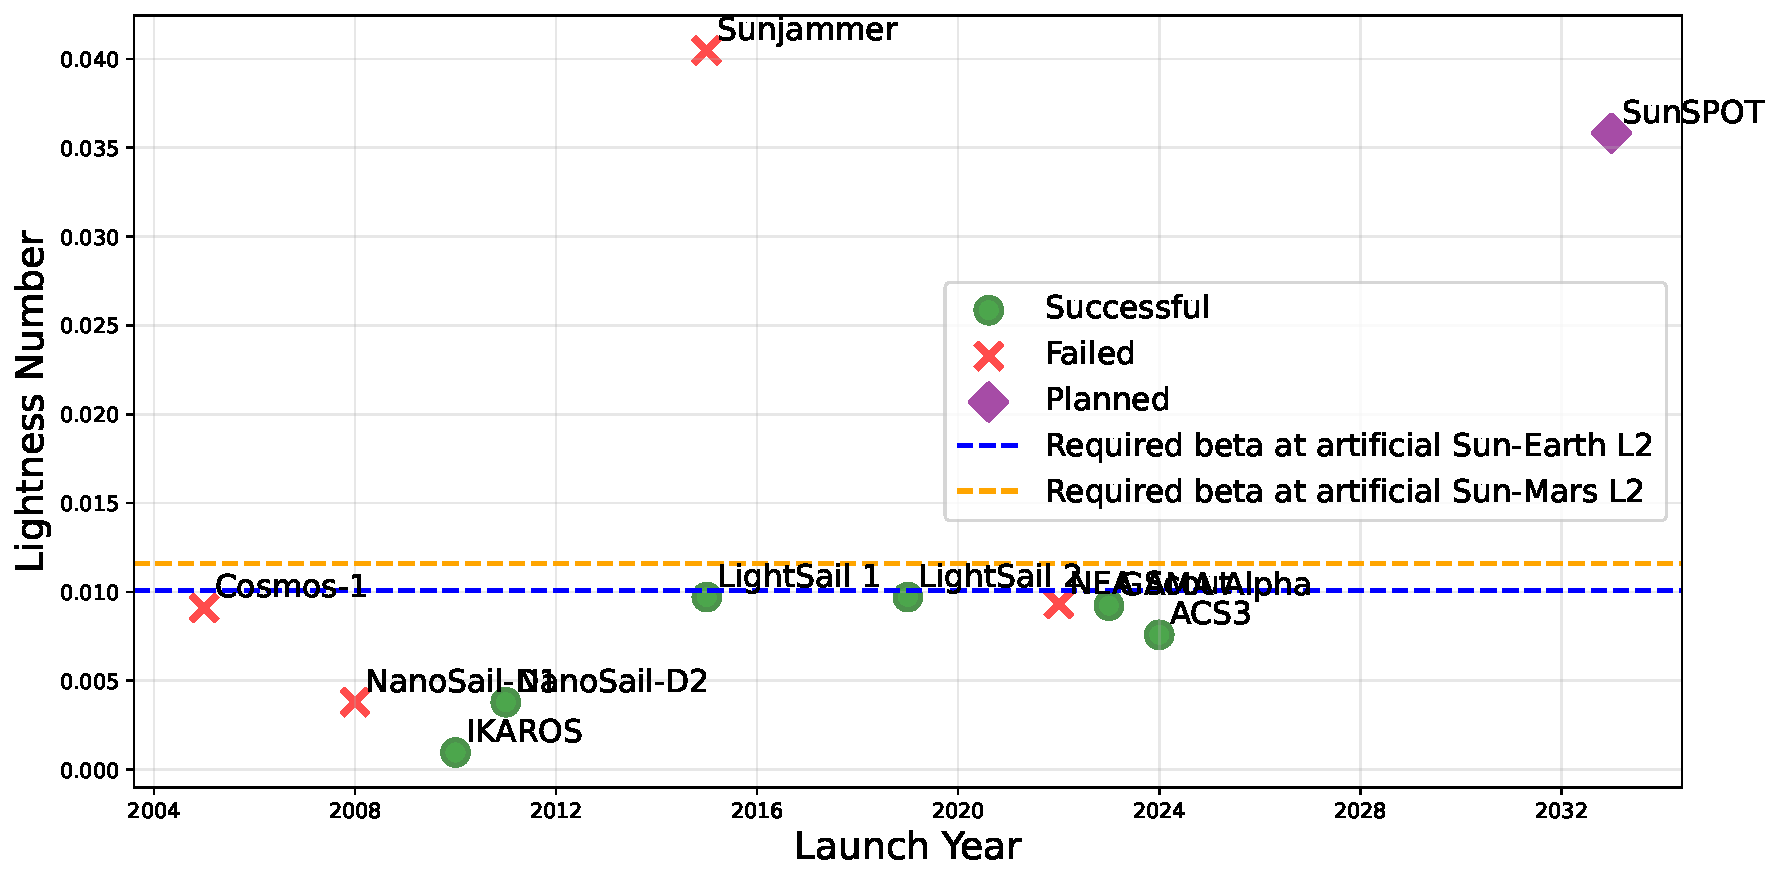
\includegraphics[width=0.8\textwidth]{../code/wps/figures/solar_sail_lightness_number.pdf}
%     \caption{Lightness number of past solar sail missions as a function of their launch year, with the required lightness number for the L2 shift required for each case.}
%     \label{fig:wp2_beta_comparison}
% \end{figure}

(41 words)

\section{Task 2.1b}

\begin{table}[H]
  \centering
  \caption{Required sail orientation to achieve the required shift in the Lagrange points of Task 2.1a.}
  \label{tab:sail_orientation}
  \begin{tabular}{@{} l c c c @{}}
    \toprule
     & $n_{x,i}$ & $n_{y,i}$ & $n_{z,i}$ \\
    \midrule
    Sun-Earth - $L_2$ & 1 & 0 & 0 \\
    Sun-Mars  - $L_2$ & 1 & 0 & 0 \\
    \bottomrule
  \end{tabular}
\end{table}

Apart from the acceleration components in \ref{sec:1.2}, the \acs{srp} acceleration is included, yielding the following expression in the rotating frame:
\begin{equation}
  \mathbf{\ddot{r}} = -2 \mathbf{\omega} \times \mathbf{\dot{r}} - \nabla U + \mathbf{a}_{\text{s}} \xRightarrow{\text{equilibrium}} 0 = -\nabla U + \mathbf{a}_{\text{s}} \Rightarrow \mathbf{a}_{\text{s}} = \nabla U,
\end{equation}
where $\mathbf{a}_{\text{s}}$ is the \acs{srp} solar-sail acceleration, expressed as
\begin{equation}
  \mathbf{a}_{\text{s}} = \beta \frac{1 - \mu}{r^2} (\mathbf{\hat{r}_1} \cdot \mathbf{\hat{n}})^2 \mathbf{\hat{n}}.
\end{equation}
Equilibrium requires $\mathbf{a}_{\text{s}} \parallel \nabla U$, meaning $\mathbf{\hat{n}}$ must be parallel to $\nabla U$. 
For an L2 shift towards the Sun, $\nabla U$ is parallel to the Sun-planet line, so the sail normal must satisfy $\mathbf{\hat{n}} \parallel x$, i.e.\ the sail is oriented perpendicular to that line.

(75 words)

\begin{figure}[H]
  \centering
  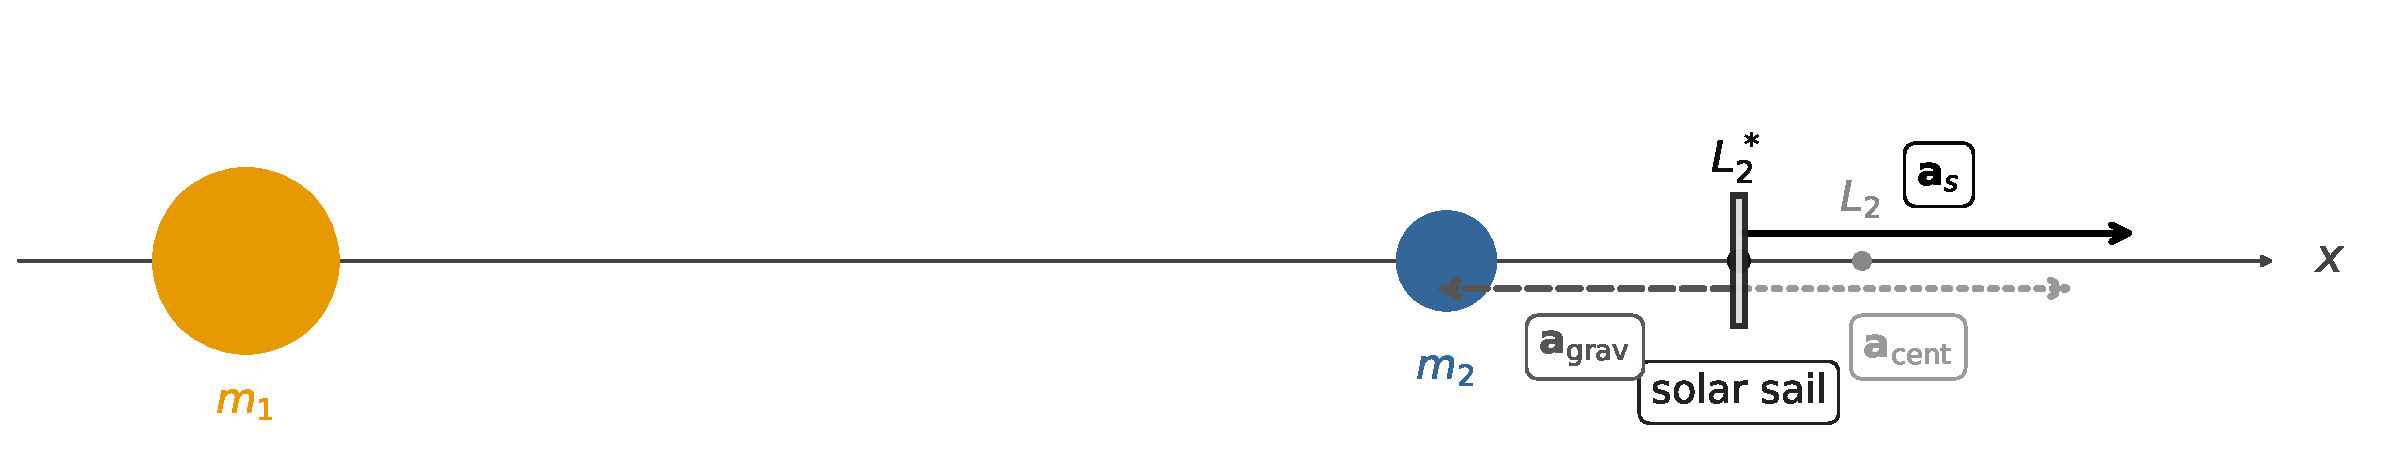
\includegraphics[width=\textwidth]{../code/wps/figures/sail_L2_schematic.pdf}
  \caption{Schematic of all acceleration vectors acting in the solar-sail augmented \ac{cr3bp}.}
  \label{fig:wp2_accel_schematic}
\end{figure}

\section{Task 2.2}
The expressions for the required $\beta$ and sail orientation are analytically derived by \textcite[217]{mcinnes1999book}. 
The validated numerical result for the lightness number is a little bit more complex, as most of the references do not tackle the exact same problem. 
However, from the values in \cite[Table~1]{heiligers2014sunjammer}, the results for the shift in L1 match up to the significant figures provided for the mass parameter. 
On a different level, since the normal vector is parallel to the gradient of the potential \parencite[eq. 5.120]{mcinnes1999book}, the required sail orientation is also verified by the fact of gradient orientation being collinear to the sun-planet line shown in \cite[Fig. 3]{mcinnes1994solar}. 

(99 words)



\section{Task 2.3}

\begin{table}[H]
  \centering
  \caption{Required solar-sail side-length to achieve the required shift in the Lagrange points of Task 2.1a.}
  \label{tab:sail_sidelength}
  \begin{tabular}{@{} l S[table-format=6.2] @{}}
    \toprule
    \textbf{Lagrange Point} & {Required solar-sail side-length [m]} \\
    \midrule
    Sun-Earth Lagrange point & 25.772 \\ % Replace with your calculated value
    Sun-Mars Lagrange point  & 27.676 \\ % Replace with your calculated value
    \bottomrule
  \end{tabular}
\end{table}
\chapter{WP3: Stability of the (artificial) Lagrange points}
\label{chapter:wp3}

\section{Task 3.1a}

\begin{table}[H]
  \centering
  \caption{Eigenvalues of the classical and artificial Lagrange points.}
  \label{tab:eigenvalues_detailed}
  \begin{tabular}{@{} l c c c c @{}}
    \toprule
    \textbf{Lagrange point} & $\lambda_1$ & $\lambda_2$ & $\lambda_3$ & $\lambda_4$ \\
    \midrule
    Sun-Earth Classical (Task 1.1a) & $3.478i$ & $-3.478i$ & $1.469$ & $-1.469$ \\
    Sun-Earth Artificial (Task 2.1a) & $3.475i$ & $-3.475i$ & $1.469$ & $-1.469$ \\
    Sun-Mars Classical (Task 1.1a) & $3.487i$ & $-3.487i$ & $1.479$ & $-1.479$ \\
    Sun-Mars Artificial (Task 2.1a) & $3.483i$ & $-3.483i$ & $1.478$ & $-1.478$ \\
    \bottomrule
  \end{tabular}
\end{table}
\chapter{WP4: Invariant manifolds and application to Mars exploration mission}
\label{chapter:wp4}

\section{Task 4.1}

\begin{figure}[H]
  \centering
  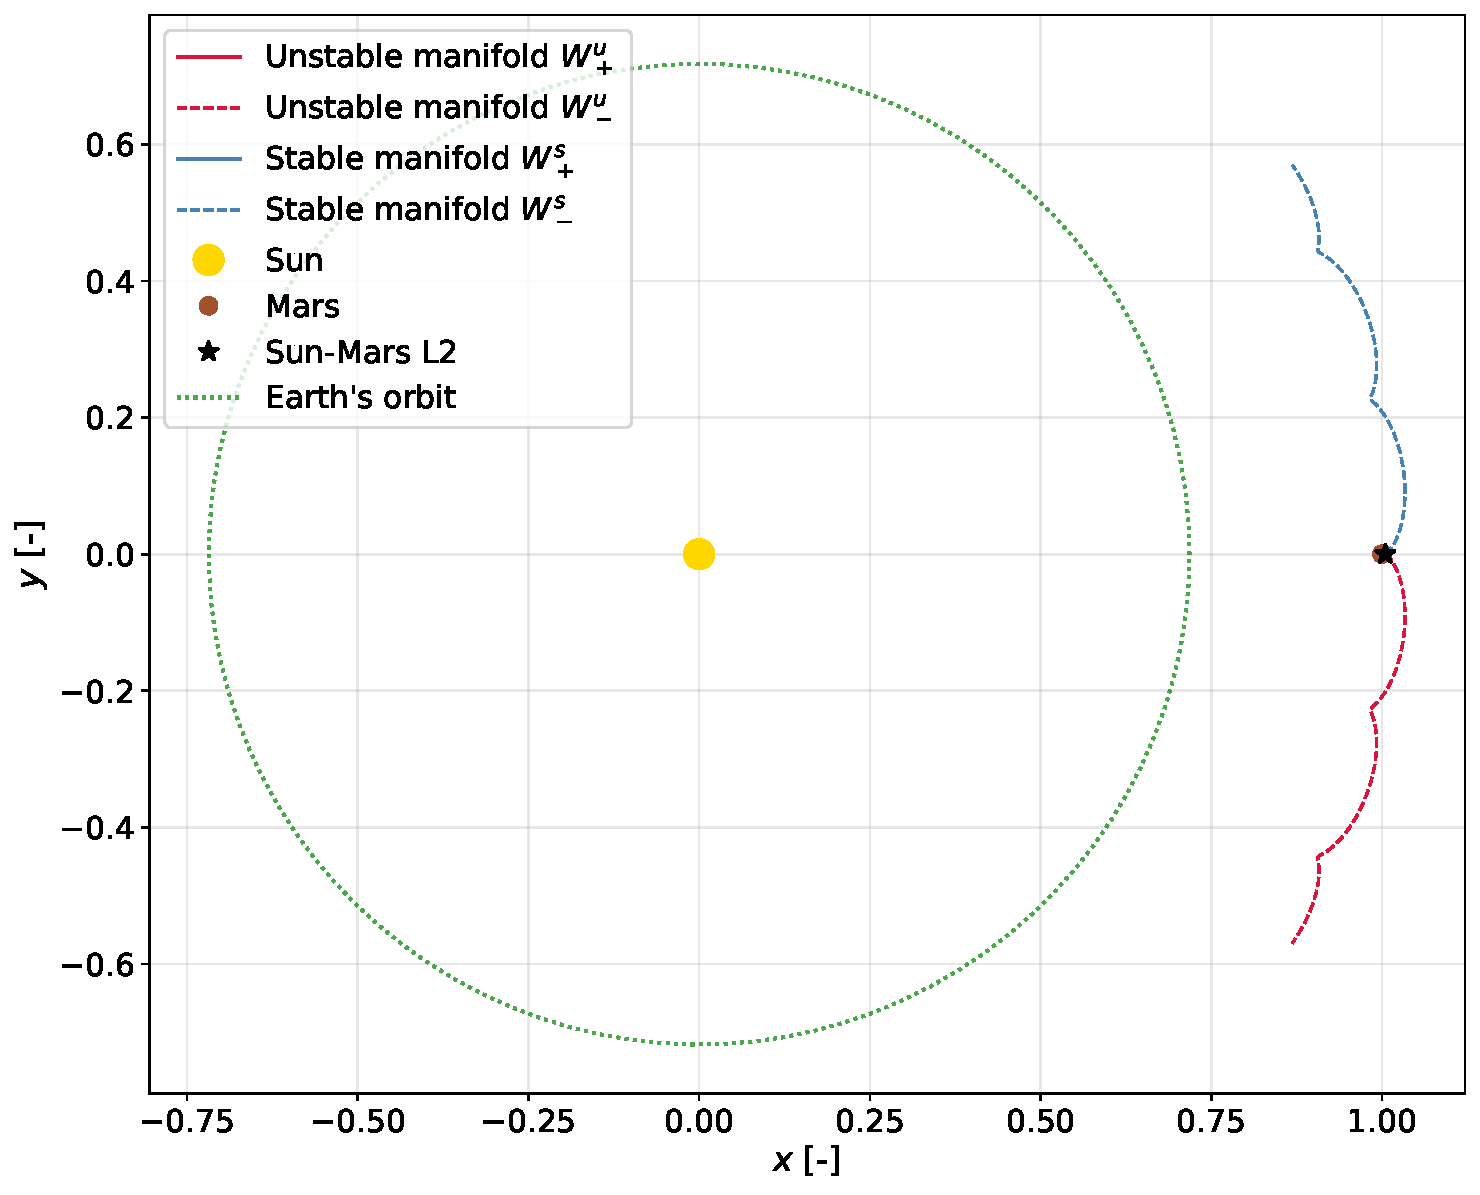
\includegraphics[width=0.65\textwidth]{../code/wps/figures/wp4_manifolds_system_wide.pdf}
  \caption{System-wide view of the invariant manifolds for the classical Sun-Mars system.}
  \label{fig:wp4_manifolds_system_wide}  
\end{figure}

\begin{figure}[H]
  \centering
  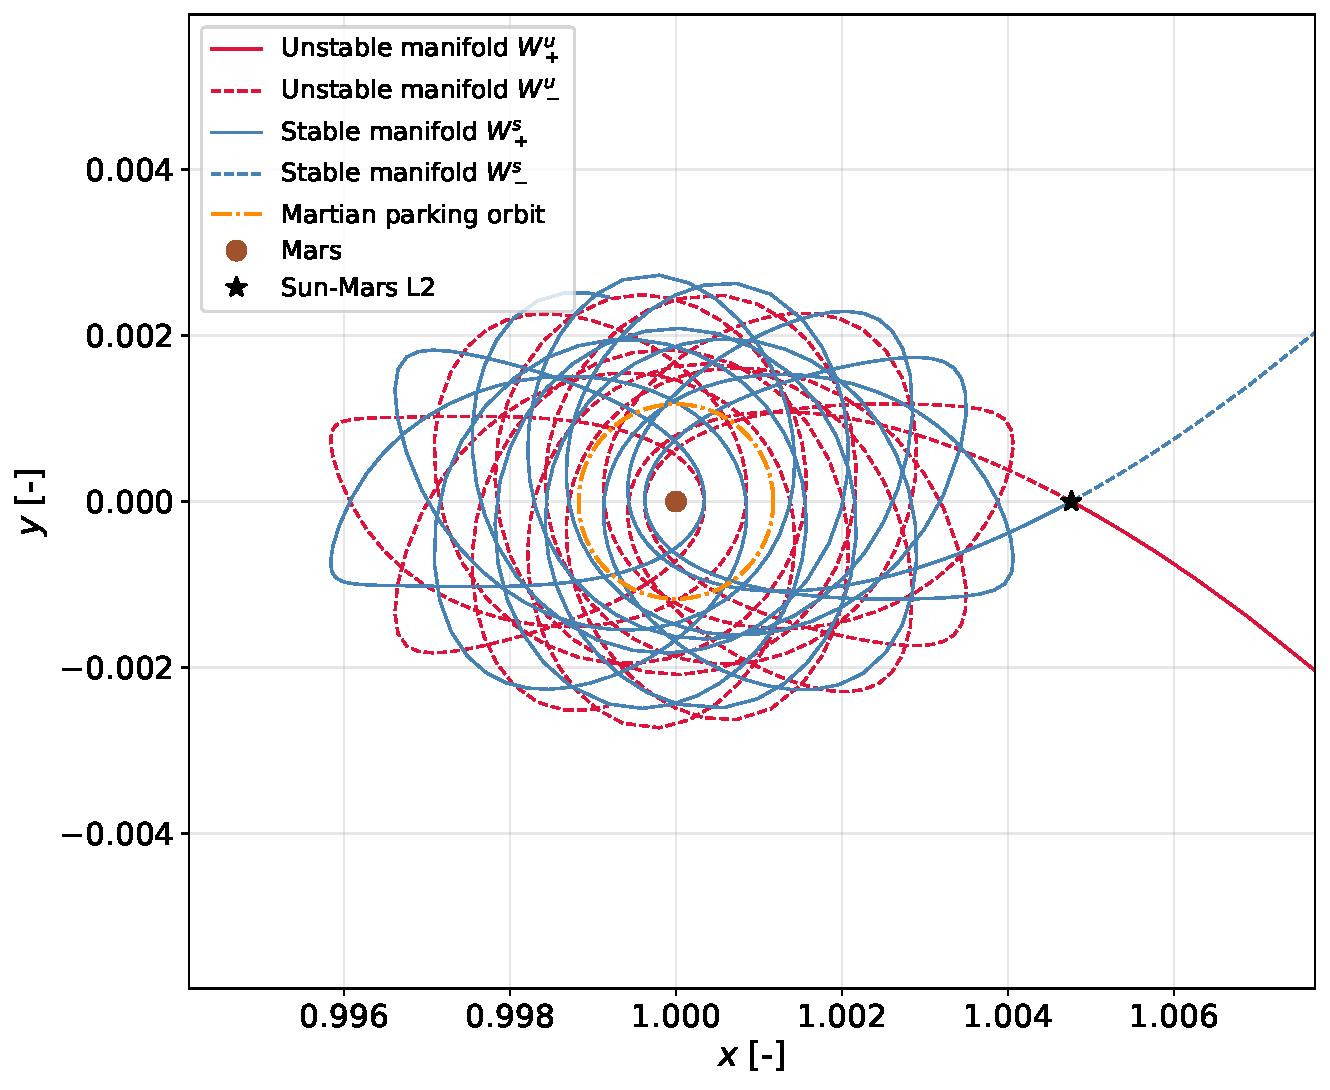
\includegraphics[width=0.65\textwidth]{../code/wps/figures/wp4_manifolds_closeup.pdf}
  \caption{Close-up view of the invariant manifolds for the classical Sun-Mars system.}
  \label{fig:wp4_manifolds_closeup}  
\end{figure}



%% Prevent urls running into margins in bibliography
\setcounter{biburlnumpenalty}{7000}
\setcounter{biburllcpenalty}{7000}
\setcounter{biburlucpenalty}{7000}

%% Add bibliography
\printbibliography[heading=bibintoc,title=References]

%% ----------------------------------------------------------------------
%%    Appendix (Letters for chapters)
%% ----------------------------------------------------------------------

\appendix

% \chapter{Derivations for WP2}
\label{chapter:derivations-wp2}

\section{Analytical approximation of the solar-sail lightness number as a function of the shift in the Lagrange points.}

For an ideal solar sail oriented normal to the Sun-line, the required lightness number $\beta$ is defined by (\parencite{mcinnes1999book}):

$$ \beta = - \frac{1}{1-\mu} \frac{dU}{dx} $$

where $\mu$ is the mass ratio and the potential gradient along the synodic $x$-axis is \parencite{mcinnes1999book}:

$$ \frac{dU}{dx} = -\frac{(1-\mu)(x+\mu)}{r_1^3} - \frac{\mu(x-(1-\mu))}{r_2^3} + x $$

We perform a first-order Taylor series expansion of the potential gradient about the $L_2$ equilibrium point. By definition:

$$ \left. \frac{dU}{dx} \right|_{x_{L2}} = 0 $$

Evaluating the gradient at the shifted position $x = x_{L2} - \delta$ yields the first-order approximation:

$$ \frac{dU}{dx}\bigg|_{x_{L2} - \delta} \approx \underbrace{\frac{dU}{dx}\bigg|_{x_{L2}}}_{=0} - \delta \cdot \frac{d^2U}{dx^2}\bigg|_{x_{L2}} + \mathcal{O}(\delta^2) $$

The expression for the required lightness number simplifies to:

$$ \beta(\delta) \approx \frac{\delta}{1-\mu} \frac{d^2U}{dx^2} $$

The second derivative of the potential characterizes the local curvature of the potential field. Differentiating the gradient with respect to $x$:

$$ \frac{d^2U}{dx^2} = \frac{d}{dx} \left( -\frac{(1-\mu)(x+\mu)}{r_1^3} - \frac{\mu(x-(1-\mu))}{r_2^3} + x \right) $$

Given that $r_1 = |x + \mu|$ and $r_2 = |x - (1-\mu)|$ for collinear points ($y=z=0$), the expression for $\frac{d^2U}{dx^2}$ is:

$$ \frac{d^2U}{dx^2} = -\frac{(1-\mu)}{r_1^3} + \frac{3(1-\mu)(x+\mu)^2}{r_1^5} - \frac{\mu}{r_2^3} + \frac{3\mu(x-(1-\mu))^2}{r_2^5} + 1 $$

At the classical $L_2$ point, $(x+\mu)^2 = r_1^2$ and $(x-(1-\mu))^2 = r_2^2$. Consequently, the terms simplify to:

$$ \frac{d^2U}{dx^2} = \left( -\frac{1-\mu}{r_1^3} + \frac{3(1-\mu)}{r_1^3} \right) + \left( -\frac{\mu}{r_2^3} + \frac{3\mu}{r_2^3} \right) + 1 $$

$$ \frac{d^2U}{dx^2} = \frac{2(1-\mu)}{r_1^3} + \frac{2\mu}{r_2^3} + 1 $$

Substituting the simplified $\frac{d^2U}{dx^2}$ into the linearized equilibrium condition, we obtain the final analytical approximation for $\beta$ as a function of the displacement $\delta$:

$$ \boxed{ \beta(\delta) = \frac{\delta}{1-\mu} \left( \frac{2(1-\mu)}{r_1^3} + \frac{2\mu}{r_2^3} + 1 \right) } $$

This linear model establishes that the required sail lightness number is directly proportional to the magnitude of the shift from the classical equilibrium. The validity of this approximation is subject to two primary constraints:
\begin{itemize}
    \item The displacement $\delta$ must be small relative to the characteristic length scale of the local potential gradient, typically $\delta \ll r_2 \approx (\mu/3)^{1/3}$.
    \item The sail acceleration vector must remain strictly collinear with the Sun-planet line to satisfy the one-dimensional assumption.
\end{itemize}
\chapter{Derivations for WP3}
\label{chapter:derivations-wp3}

\section{Stability analysis of the trivial CR3BP ($\mu = 0$)}
\label{sec:trivial-cr3bp}

To verify the implementation of the Jacobian matrix, the trivial case $\mu = 0$ is considered analytically. With $\mu = 0$, the effective potential reduces to (\parencite{wakker2015fundamentals}):

$$
U \xrightarrow{\;\mu \to 0\;} \frac{1}{2}(x^2 + y^2) + \frac{1}{r_1}, \qquad r_1 = \sqrt{x^2 + y^2}
$$

The first partial derivatives of $U$ are:

$$
\frac{\partial U}{\partial x} = x - \frac{x}{r_1^3}, \qquad \frac{\partial U}{\partial y} = y - \frac{y}{r_1^3}
$$

The gradient can be written as:

$$
\nabla U = \begin{bmatrix} x \\ y \end{bmatrix} \left( -1 + \frac{1}{r_1^3} \right)
$$

By definition, at the Lagrange points $\nabla U = \mathbf{0}$. For $[x,\,y]^{\top} \neq \mathbf{0}$ this requires $r_1 = 1$, so all three collinear Lagrange points collapse to $x = 1$.

The second partial derivatives of $U$ are:

$$
U_{xx} = 1 - \frac{1}{r_1^3} + \frac{3x^2}{r_1^5}, \qquad U_{xy} = \frac{3xy}{r_1^5}, \qquad U_{yy} = 1 - \frac{1}{r_1^3} + \frac{3y^2}{r_1^5}
$$

Evaluating at $x = 1,\; y = 0$ (so $r_1 = 1$):

$$
U_{xx} = 1 - 1 + 3 = 3, \qquad U_{xy} = 0, \qquad U_{yy} = 1 - 1 + 0 = 0
$$

The linearised equations of motion around the libration point, with state vector $\boldsymbol{s} = [x',\, y',\, \dot{x}',\, \dot{y}']^{\top}$, take the form $\dot{\boldsymbol{s}} = \mathbf{A}\,\boldsymbol{s}$ (\parencite{wakker2015fundamentals}, Eq.~3.86):

$$
\mathbf{A} =
\begin{bmatrix}
    0      & 0      & 1  & 0 \\
    0      & 0      & 0  & 1 \\
    U_{xx} & U_{xy} & 0  & 2 \\
    U_{xy} & U_{yy} & -2 & 0
\end{bmatrix}
=
\begin{bmatrix}
    0 & 0 &  1 & 0 \\
    0 & 0 &  0 & 1 \\
    3 & 0 &  0 & 2 \\
    0 & 0 & -2 & 0
\end{bmatrix}
$$

Substituting into the characteristic polynomial (\parencite{wakker2015fundamentals}, Eq.~3.90):

$$
\lambda^4 + \bigl(4 - U_{xx} - U_{yy}\bigr)\,\lambda^2 + U_{xx}\,U_{yy} - U_{xy}^2 = 0
$$

yields, with $U_{xx} = 3$, $U_{yy} = 0$, $U_{xy} = 0$:

$$
\lambda^4 + \lambda^2 = 0 \quad\Longrightarrow\quad \lambda^2\!\left(\lambda^2 + 1\right) = 0 
$$

The four eigenvalues are therefore:

$$
\lambda_{1,2} = \pm\,i, \qquad \lambda_{3,4} = 0
$$

All eigenvalues have non-positive real parts. The purely imaginary pair $\pm i$ corresponds to a neutrally stable oscillation at the non-dimensional frequency $\omega = 1$ (one orbital period), while the double zero eigenvalue reflects the degenerate centre structure of the trivial case. The libration point is therefore \emph{marginally stable} for $\mu = 0$, consistent with the analytical expectation that in the absence of a secondary body all perturbations reduce to circular orbital motion about the primary.
\chapter{Derivations for WP4}
\label{chapter:derivations-wp4}

\section{Acceleration of the sail for the planar \ac{eom}} 
\label{section:acceleration-sail-eom}

From \cite[section 2.2.3]{mcinnes2000strategies}, the \ac{eom} in the solar-sail augmented \ac{cr3bp} are taken and adapted to our planar case. 

From the most general case of the solar sail acceleration \parencite[eq. 2.53]{mcinnes2000strategies}:

\begin{equation}
    \mathbf{a_\text{sail}} = \beta \frac{1 - \mu}{r_1^2} \cos^2\!\alpha \; \mathbf{\hat{n}}
\end{equation}

The components of the acceleration are then given by \cite[eq. 2.58-2.60]{mcinnes2000strategies}:

\begin{align}
    a_x &= \beta \,\frac{1-\mu}{r_1^2} \cos^2\!\alpha \; n_x \\
    a_y &= \beta \,\frac{1-\mu}{r_1^2} \cos^2\!\alpha \; n_y \\
    a_z &= \beta \,\frac{1-\mu}{r_1^2} \cos^2\!\alpha \; n_z
\end{align}

And the components of the unit vector $\mathbf{\hat{n}}$ are given by \cite[eq. 2.54-2.56]{mcinnes2000strategies}:

\begin{align}
n_x &= \frac{\cos\alpha\,(x+\mu)}{|\vec{r}_1|} - \frac{\sin\alpha\cos\gamma\,(x+\mu)\,z}{|(\vec{r}_1\times\hat{z})\times\vec{r}_1|} + \frac{\sin\alpha\sin\gamma\, y}{|\vec{r}_1\times\hat{z}|} \\
n_y &= \frac{\cos\alpha\, y}{|\vec{r}_1|} - \frac{\sin\alpha\cos\gamma\, y\,z}{|(\vec{r}_1\times\hat{z})\times\vec{r}_1|} - \frac{\sin\alpha\sin\gamma\,(x+\mu)}{|\vec{r}_1\times\hat{z}|} \\
n_z &= \frac{\cos\alpha\, z}{|\vec{r}_1|} + \frac{\sin\alpha\cos\gamma\,(y^2+(x+\mu)^2)}{|(\vec{r}_1\times\hat{z})\times\vec{r}_1|},
\end{align}

where $\alpha$ and $\gamma$ are the cone and clock angles, respectively.

Hence, the augmented \ac{eom} are:

\begin{align}
\ddot{x} - 2\dot{y} &= U_x + a_x \\
\ddot{y} + 2\dot{x} &= U_y + a_y \\
\ddot{z} &= U_z + a_z
\end{align}

In our case, we have a planar problem ($z=0$) and, out of the assignment's requirements, it is chosen $\gamma = 90^{\circ}$

\begin{align}
n_x &= \frac{\cos\alpha\,(x+\mu) + \sin\gamma\, y}{r_1} \\
n_y &= \frac{\cos\alpha\, y - \sin\alpha\,(x+\mu)}{r_1} \\
n_z &= 0
\end{align}

It can be shown that, for the trivial $\alpha = 0$ case considered before, the expressions in the equations avobe simplify to:

\begin{align}
a_x &= \beta \,\frac{(1-\mu) (x+\mu)}{r_1^2} \\
a_y &= 0 \\
a_z &= 0
\end{align}
\chapter{AI Usage appendix}
\label{chapter:ai-usage}

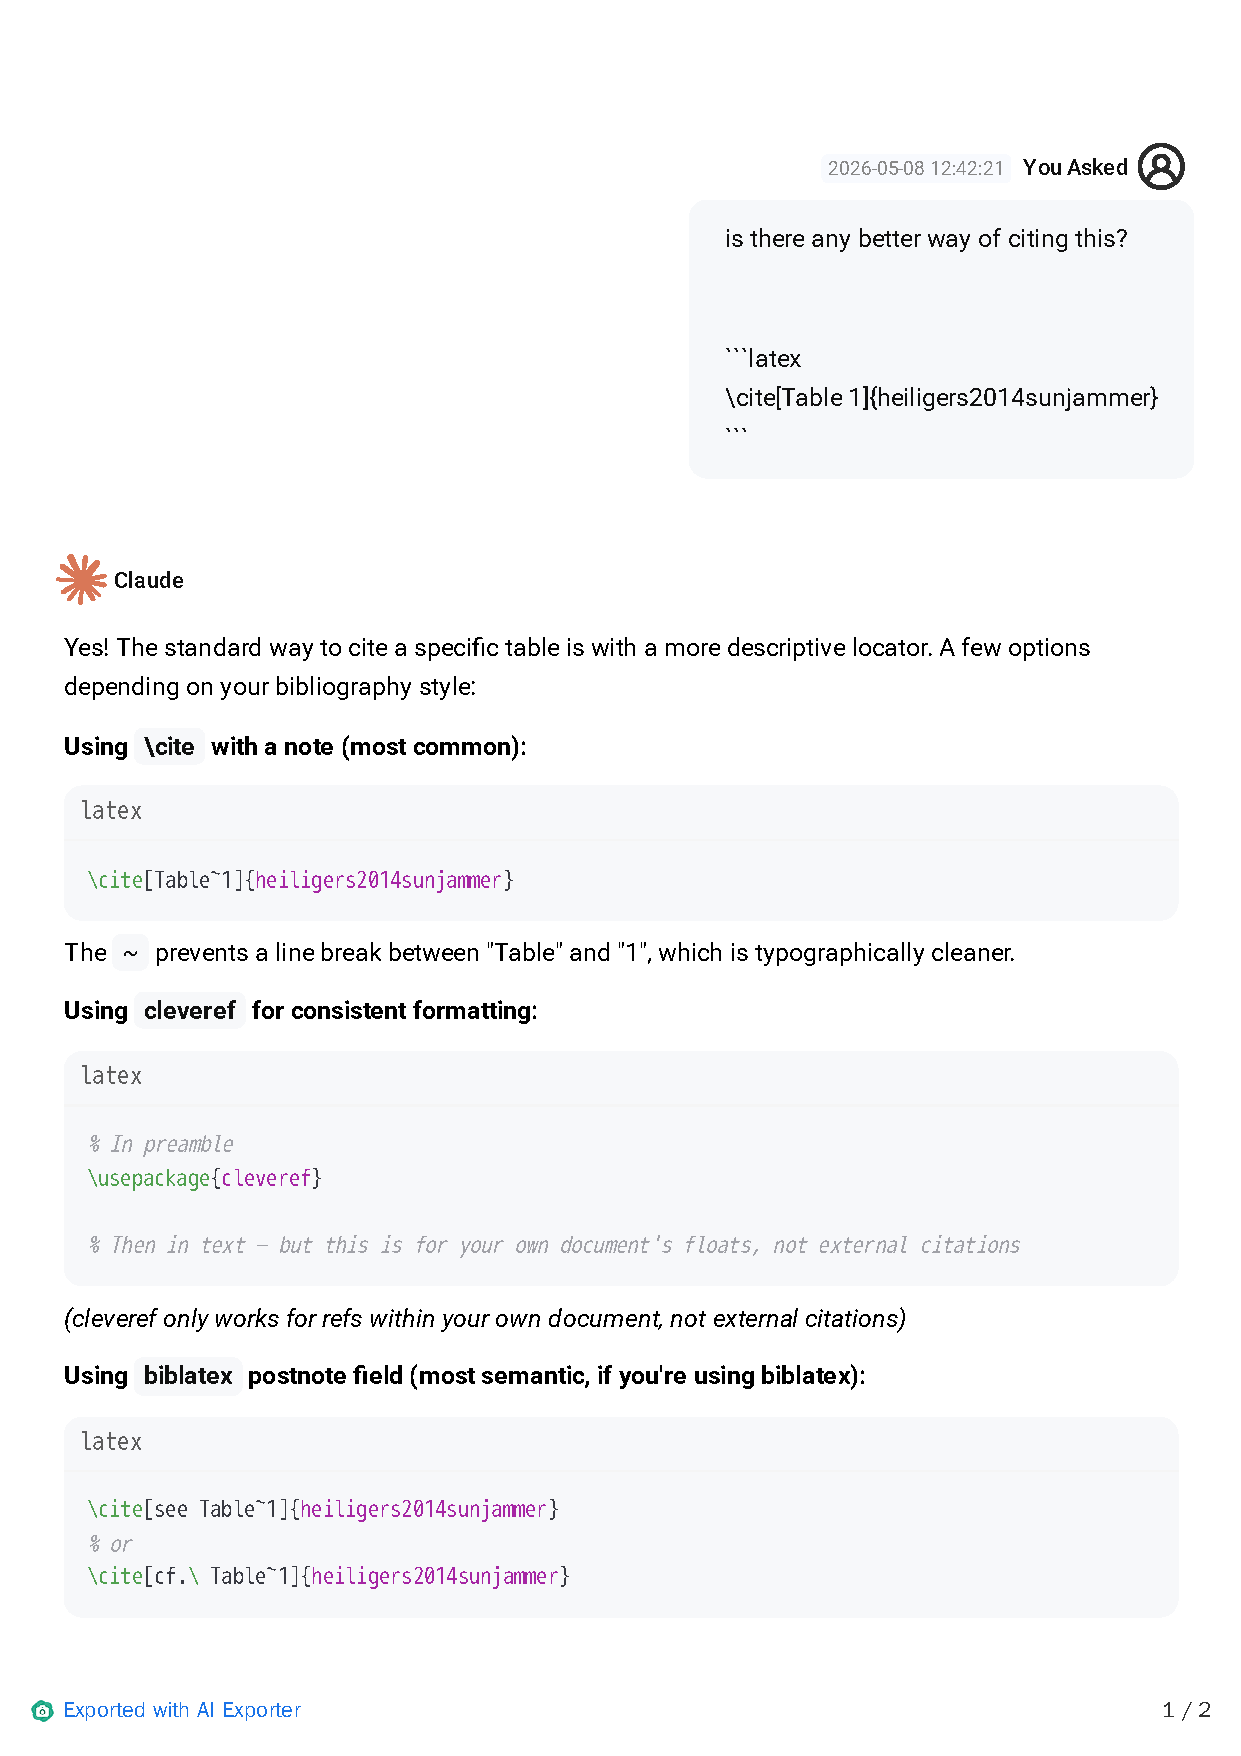
\includepdf[pages=-,pagecommand={},scale=0.95,frame=false]{ai_usage/Claude1.pdf}
 % Create file to add

\end{document}
